\documentclass[aspectratio=169]{beamer}
\usepackage{graphicx}
\usepackage{xcolor}
\usepackage{amsmath}
\usepackage{upgreek}
\usepackage{tikz}
\usetikzlibrary{arrows.meta,positioning}

% Nord-inspired slide colors
\definecolor{NordBody}{HTML}{4C566A}
\definecolor{NordBlue}{HTML}{5E81AC}

% Custom footline with slide numbers in bottom left
\setbeamertemplate{footline}{
  \hspace{1em}%
  \usebeamercolor[fg]{page number in head/foot}%
  \usebeamerfont{page number in head/foot}%
  \insertframenumber\,/\,\inserttotalframenumber%
  \vskip2pt%
}

\beamertemplatenavigationsymbolsempty

% Text-color theme
\setbeamercolor{normal text}{fg=NordBody}
\setbeamercolor{title}{fg=NordBlue}
\setbeamercolor{frametitle}{fg=NordBlue}
\setbeamercolor{structure}{fg=NordBlue}
\setbeamercolor{itemize/enumerate body}{fg=NordBody}
\setbeamercolor{itemize/enumerate subbody}{fg=NordBody}
\setbeamercolor{itemize/enumerate subsubbody}{fg=NordBody}
\setbeamercolor{itemize item}{fg=NordBlue}
\setbeamercolor{itemize subitem}{fg=NordBlue}
\setbeamercolor{itemize subsubitem}{fg=NordBlue}
\setbeamercolor{enumerate item}{fg=NordBlue}
\setbeamercolor{enumerate subitem}{fg=NordBlue}
\setbeamercolor{enumerate subsubitem}{fg=NordBlue}

% Global hyperlink style
\hypersetup{
  colorlinks=true,
  allcolors=NordBlue
}

\title{Compact and Fast ADCs for Pixel Detectors}
\author{Kennedy Caisley, Hans Kr\"uger, Jochen Dingfelder}
\institute{University of Bonn}
\date{DPG 2026}

\begin{document}

%% ============================================================
%% Title
%% ============================================================
\begin{frame}
  \titlepage
  \vfill
  \begin{center}
    
\includegraphics[height=1.3cm]{images/logo_bonn.jpg}%
    \hspace{0.8cm}%
    
\includegraphics[height=1.3cm]{images/logo_ftd.jpg}%
    \hspace{0.8cm}%
    
\includegraphics[height=1.43cm]{images/logo_silab.png}%
  \end{center}
\end{frame}

%% ============================================================
%% Motivation: Detector & Hit Rate
%% ============================================================
\begin{frame}
  \frametitle{Pixel Detectors \& Hit Rates}
  \vspace{-0.3cm}
  \begin{columns}
    \begin{column}{0.6\textwidth}
      \begin{center}
        \includegraphics[width=\linewidth,height=0.88\textheight,keepaspectratio]{../phys/results/hit_rate_vs_fluence.png}
      \end{center}
    \end{column}
    \begin{column}{0.4\textwidth}
      \begin{center}
        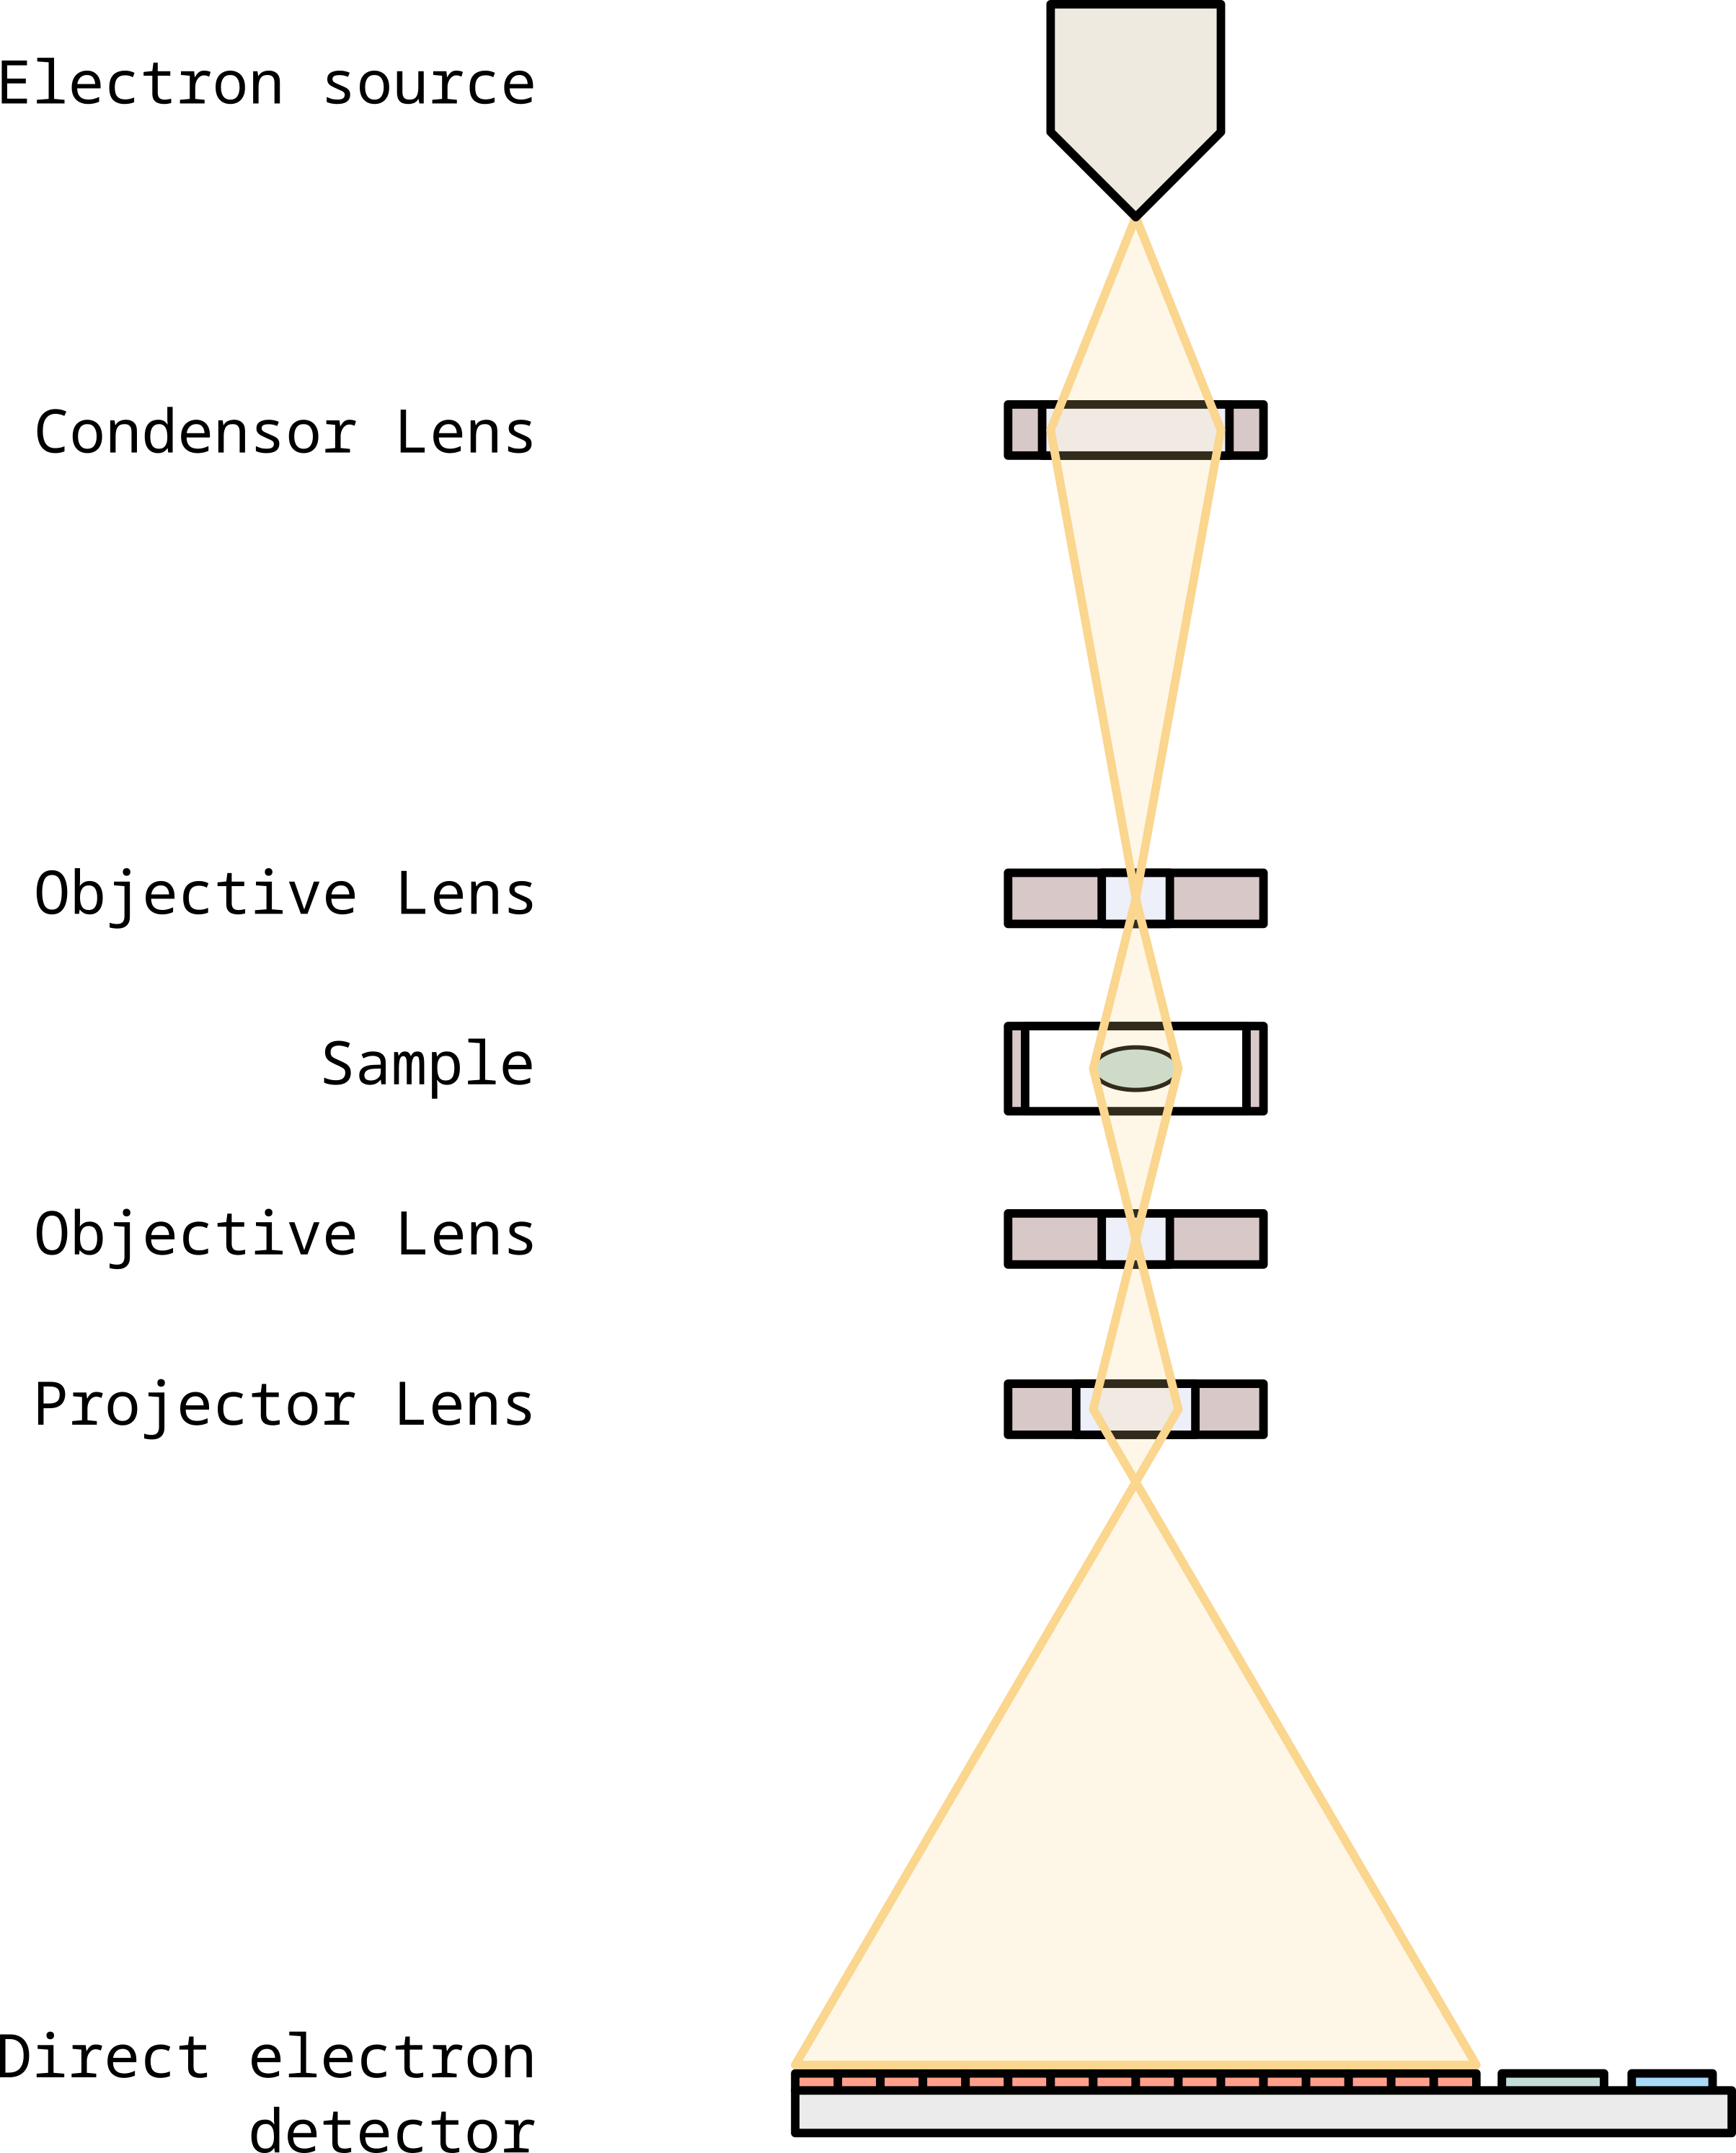
\includegraphics[height=0.72\textheight,keepaspectratio]{images/tem.png}
      \end{center}
    \end{column}
  \end{columns}
\end{frame}

%% ============================================================
%% Counting Rate & ADC System
%% ============================================================
\begin{frame}
  \frametitle{Integrating vs Discriminating Detectors}
  \vspace{-0.3cm}
  \begin{center}
    \includegraphics[width=\linewidth,height=0.48\textheight,keepaspectratio]{../phys/results/max_counting_rate_vs_window.png}
  \end{center}
  \vspace{-0.2cm}
  \begin{center}
    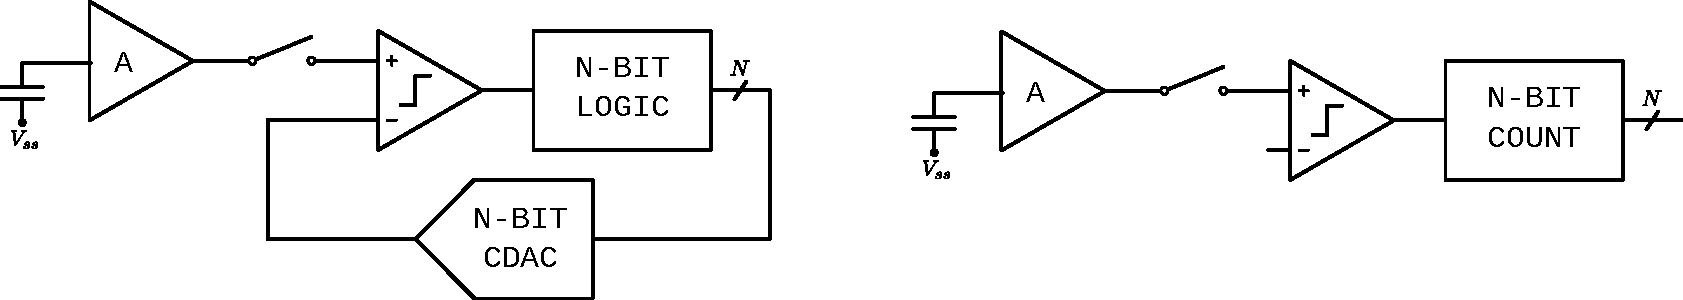
\includegraphics[width=\linewidth,height=0.38\textheight,keepaspectratio]{images/adc_system.pdf}
  \end{center}
\end{frame}

%% ============================================================
%% System Architecture
%% ============================================================
\begin{frame}
  \frametitle{System Architecture}
  \begin{center}
    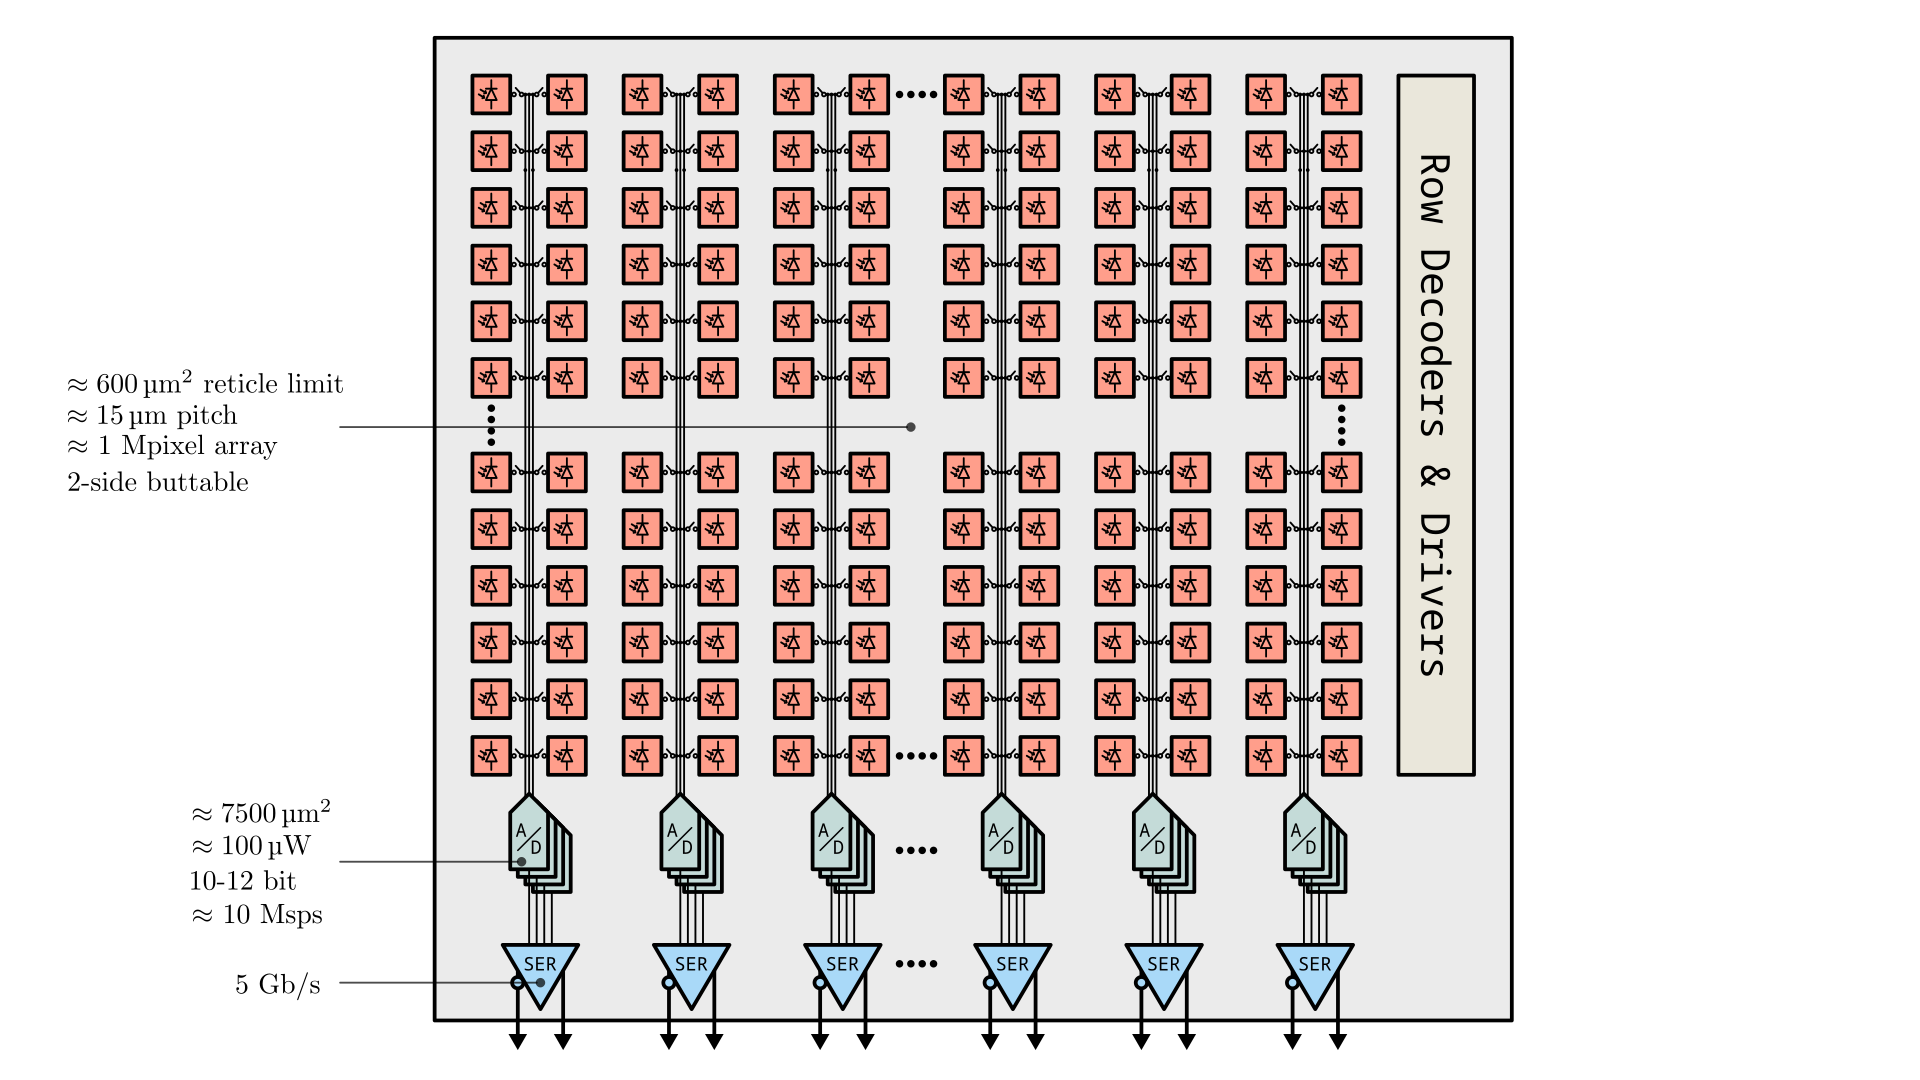
\includegraphics[width=0.85\linewidth,height=0.85\textheight,keepaspectratio]{images/arch.png}
  \end{center}
\end{frame}

%% ============================================================
%% Cross Section (hidden)
%% ============================================================
% \begin{frame}
%   \frametitle{Detector Cross Section}
%   \begin{center}
%     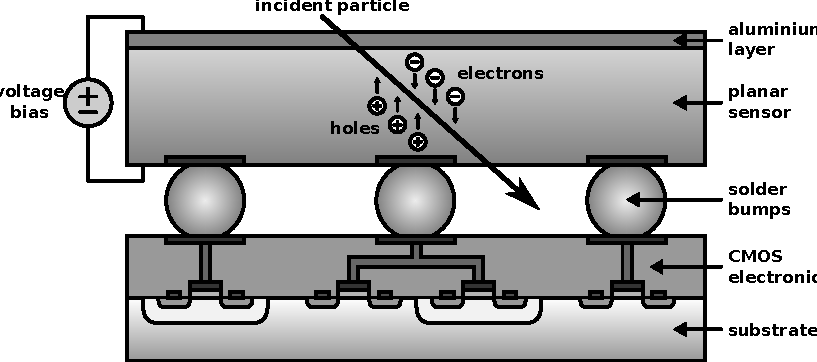
\includegraphics[width=0.85\linewidth,height=0.85\textheight,keepaspectratio]{images/cross_section.pdf}
%   \end{center}
% \end{frame}

%% ============================================================
%% ADC Block Diagram + Sub-blocks
%% ============================================================
\begin{frame}
  \frametitle{SAR ADC Architecture}
  % Top row: comparator | block diagram | digital
  \vspace{-0.2cm}
  \begin{columns}[T]
    \begin{column}{0.20\textwidth}
      \vspace{0.3cm}
      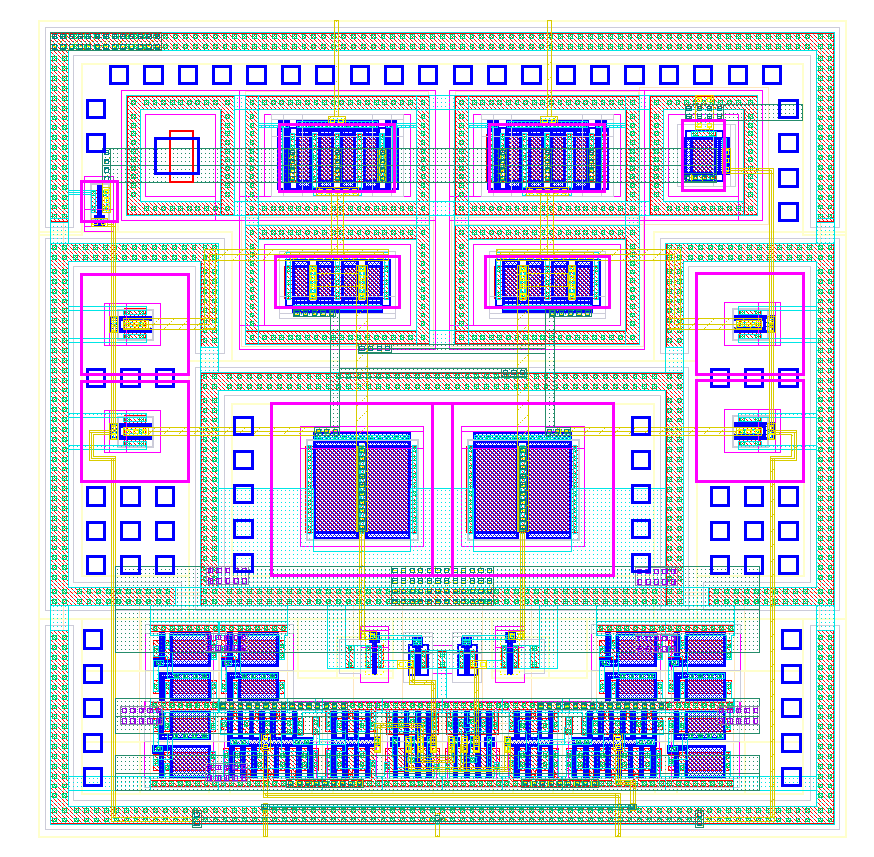
\includegraphics[width=\linewidth]{images/frida_comp.png}\\[2pt]
      {\tiny\fontsize{5}{5.5}\selectfont\lineskiplimit=-\maxdimen \textbf{Comparator:}\\
      \textbullet~$<$100\,$\upmu$V$_{\mathrm{rms}}$ noise\\
      \textbullet~$<$20\,$\upmu$W power\\
      \textbullet~$<$2\,ns metastability\\}
    \end{column}
    \begin{column}{0.55\textwidth}
      \begin{center}
        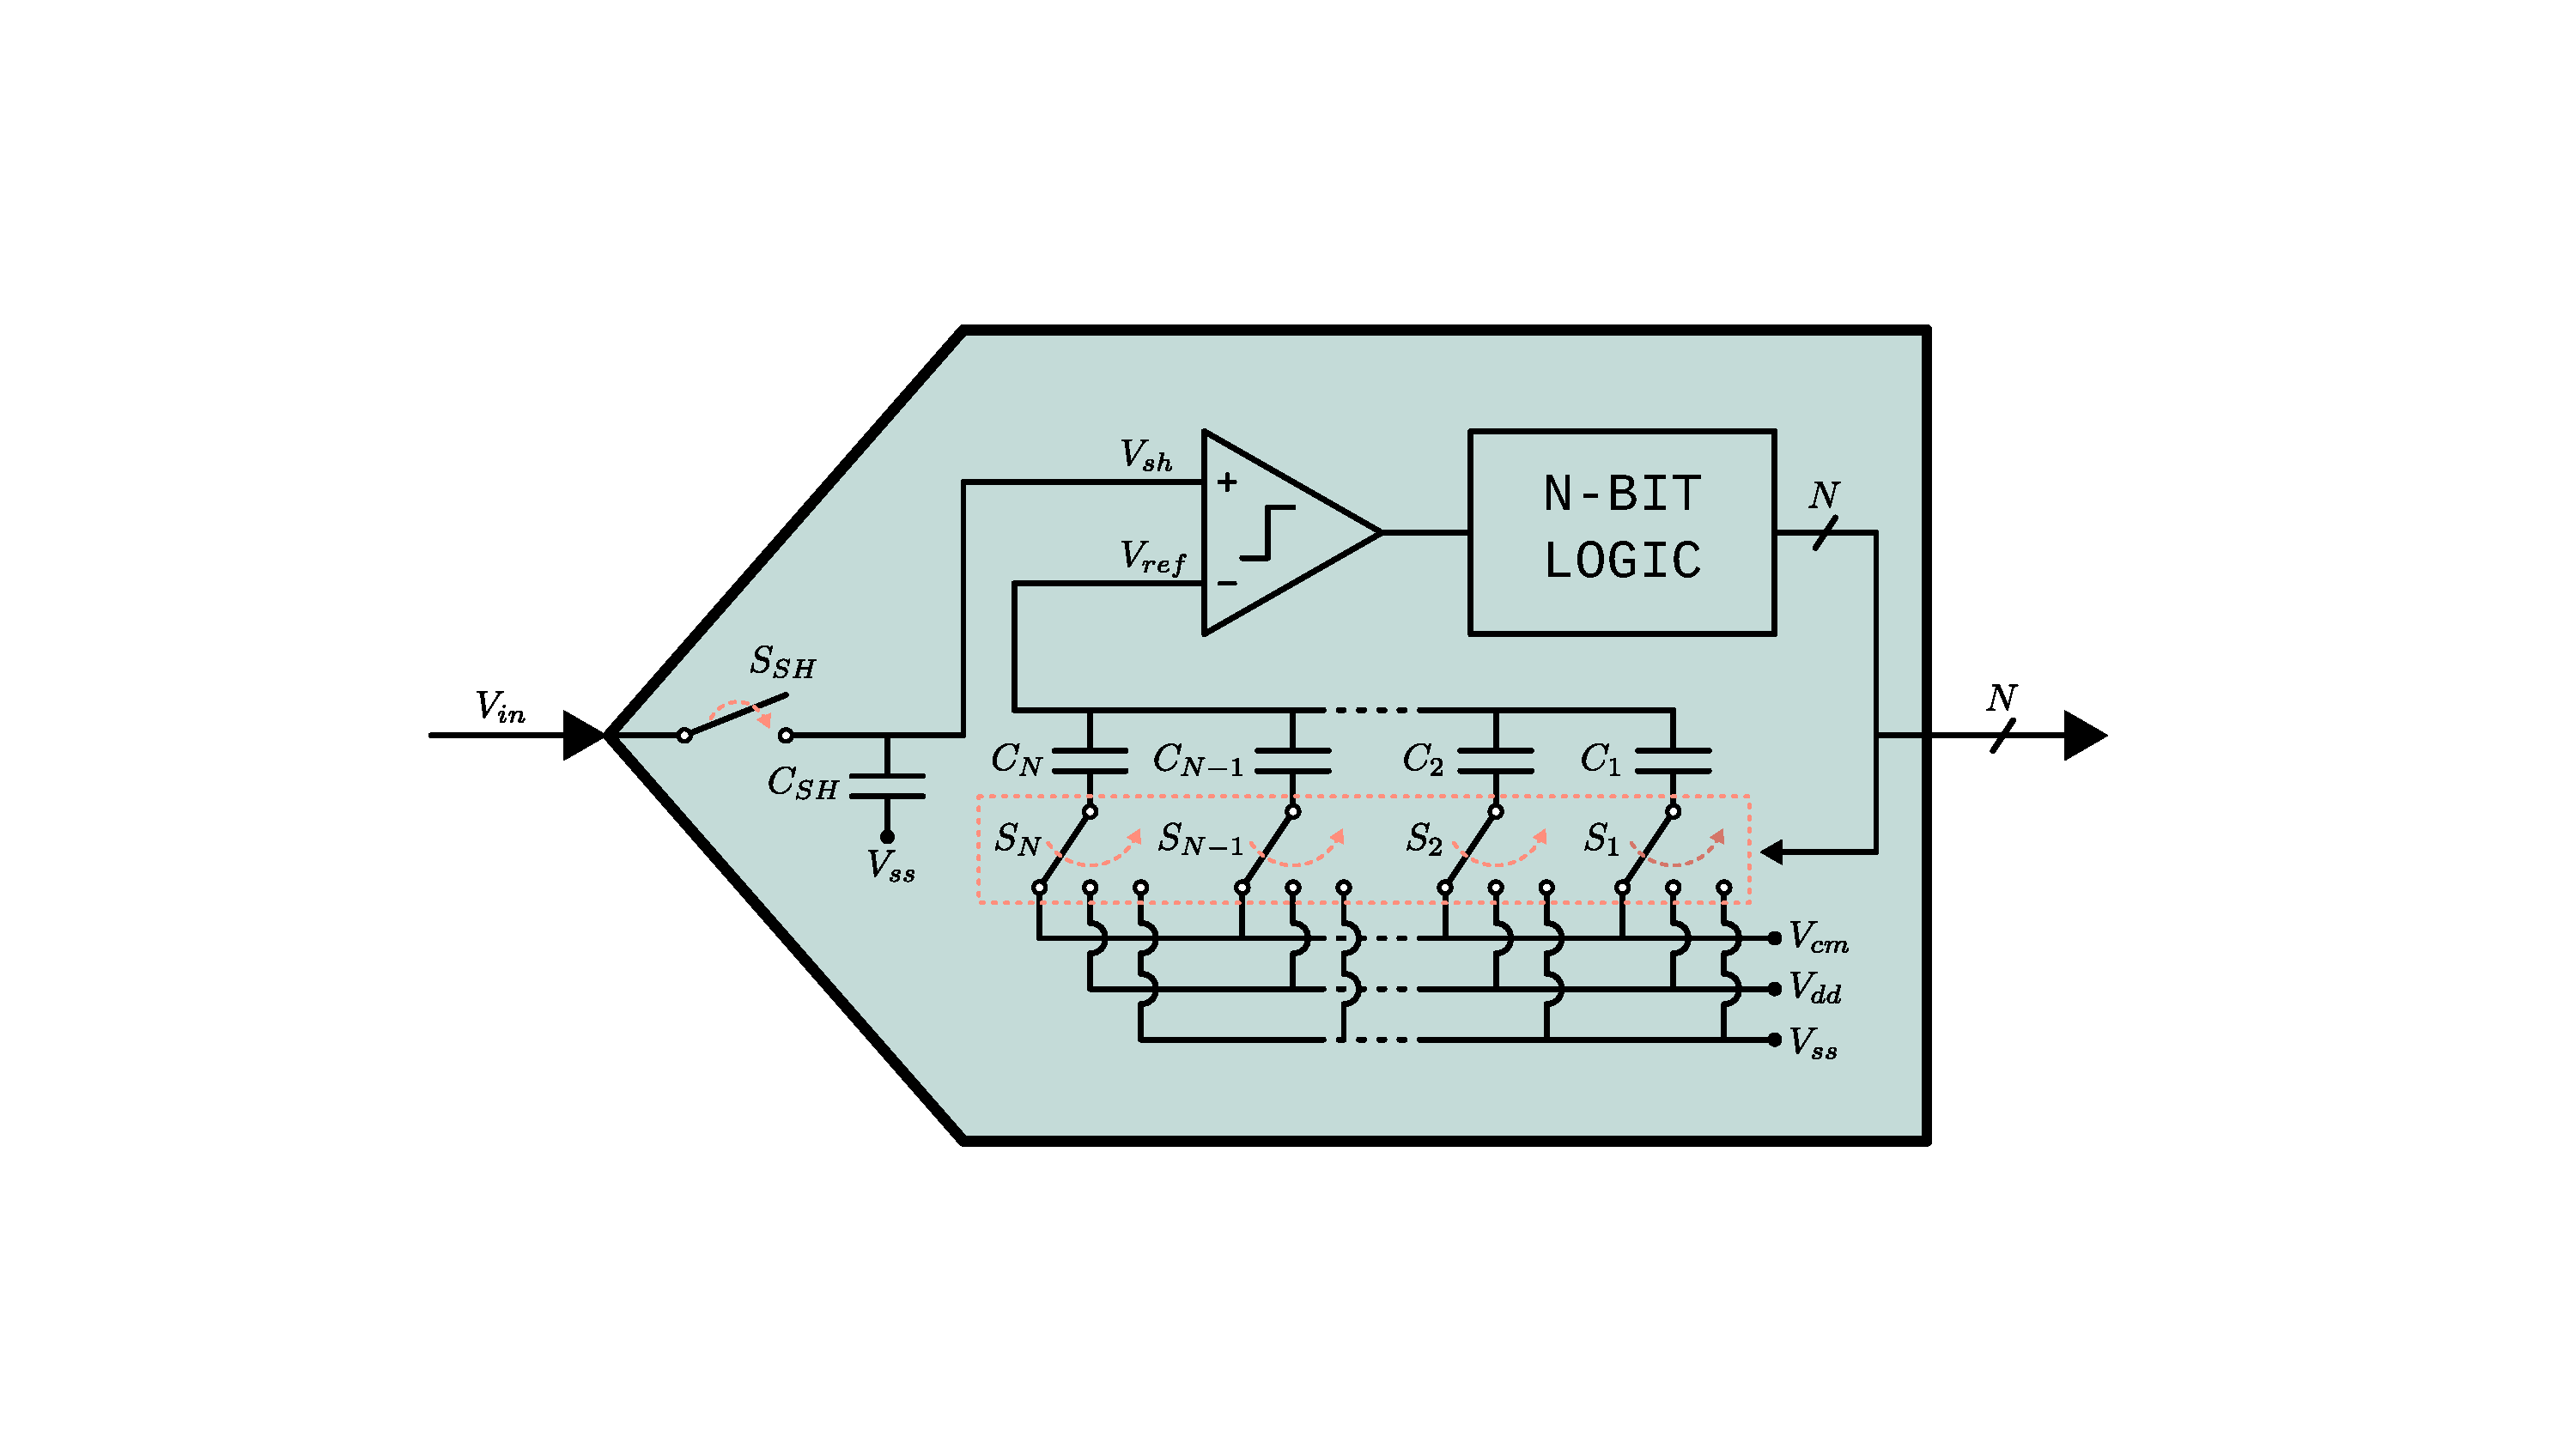
\includegraphics[width=\linewidth]{images/adc_basic.pdf}
      \end{center}
    \end{column}
    \begin{column}{0.30\textwidth}
      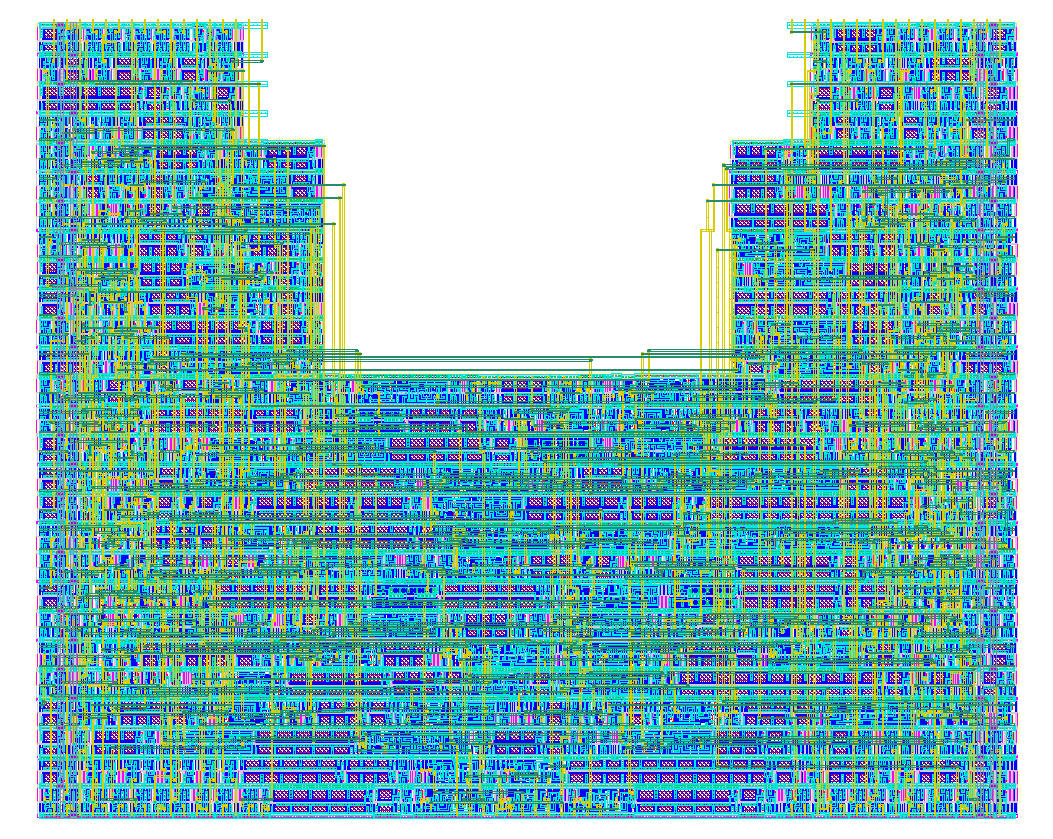
\includegraphics[width=\linewidth]{images/frida_adc_dgital.png}\\[2pt]
      {\tiny\fontsize{5}{5.5}\selectfont\lineskiplimit=-\maxdimen \textbf{SA Digital Logic:}\\
      \textbullet~17-bit state machine\\
      \textbullet~Manual bit ctrl for testing\\
      \textbullet~Programmable init.\ state\\}
    \end{column}
  \end{columns}
  \vspace{-0.1cm}
  % Bottom row: switch | CDAC unit | cap driver
  \begin{columns}[T]
    \begin{column}{0.16\textwidth}
      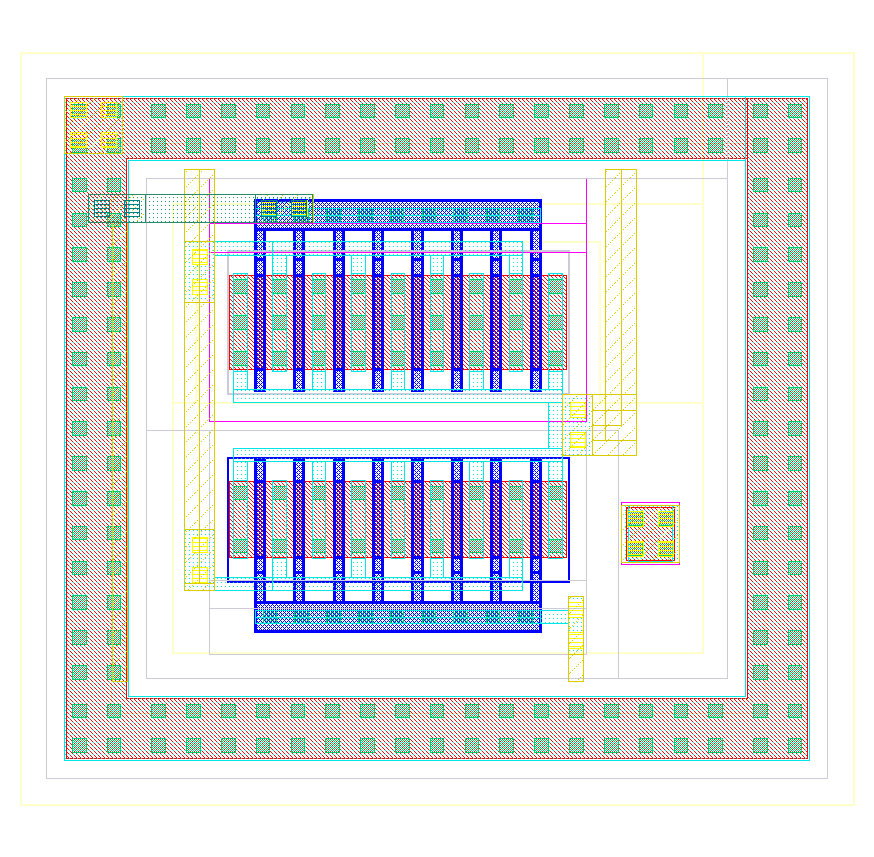
\includegraphics[width=\linewidth,height=2cm,keepaspectratio]{images/frida_samp.png}\\[2pt]
      {\tiny\fontsize{5}{5.5}\selectfont\lineskiplimit=-\maxdimen \textbf{Samp.\ Switch:}\\
      \textbullet~200\,MHz BW\\
      \textbullet~No bootstrap\\
      \textbullet~$<$1\,k$\Omega$ $R_{\mathrm{on}}$\\}
    \end{column}
    \begin{column}{0.10\textwidth}
      \mbox{}
    \end{column}
    \begin{column}{0.14\textwidth}
      \vspace{0.3cm}
      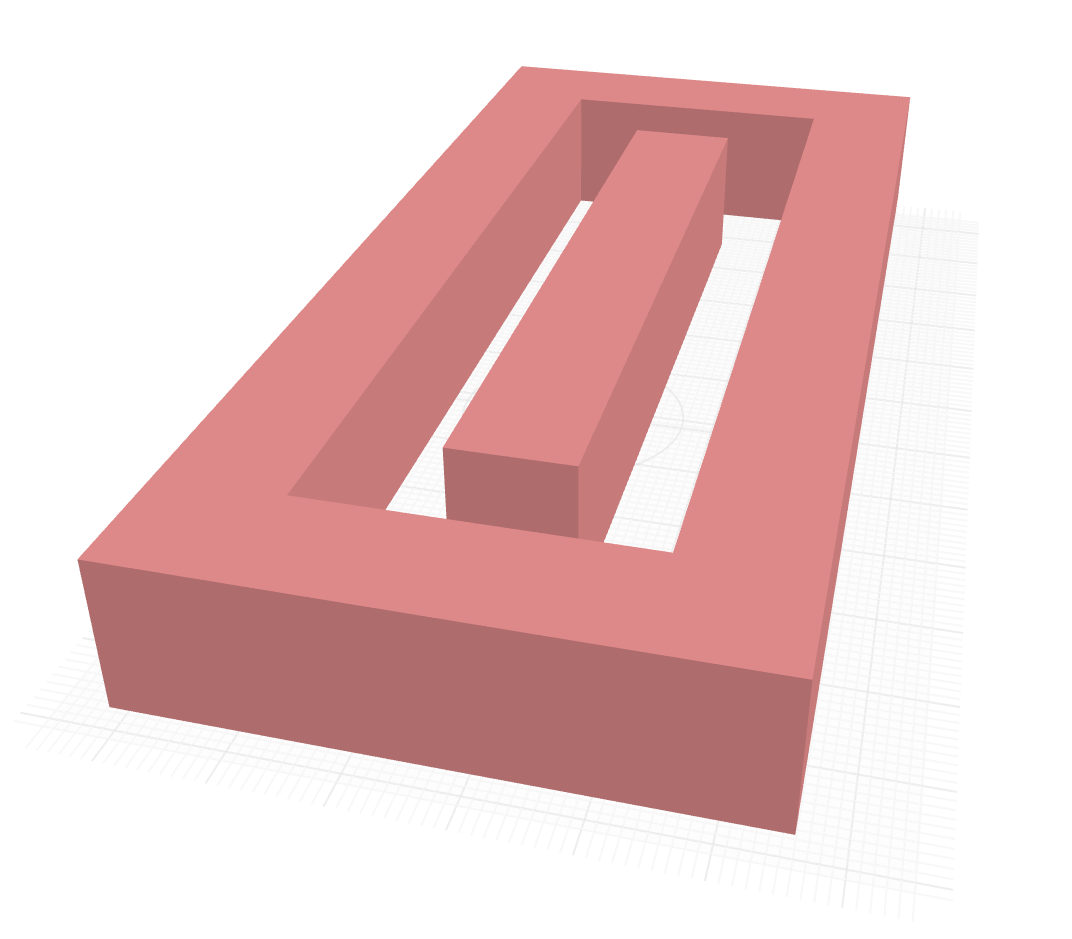
\includegraphics[width=\linewidth,height=2cm,keepaspectratio]{images/cdac_unit_cell_3d.png}\\[2pt]
      {\tiny\fontsize{5}{5.5}\selectfont\lineskiplimit=-\maxdimen \textbf{CDAC:}\\
      \textbullet~1.6\,pF total\\
      \textbullet~0.4\,aF unit\\
      \textbullet~M5--M7 fringe\\}
    \end{column}
    \begin{column}{0.39\textwidth}
      \vspace{0.3cm}
      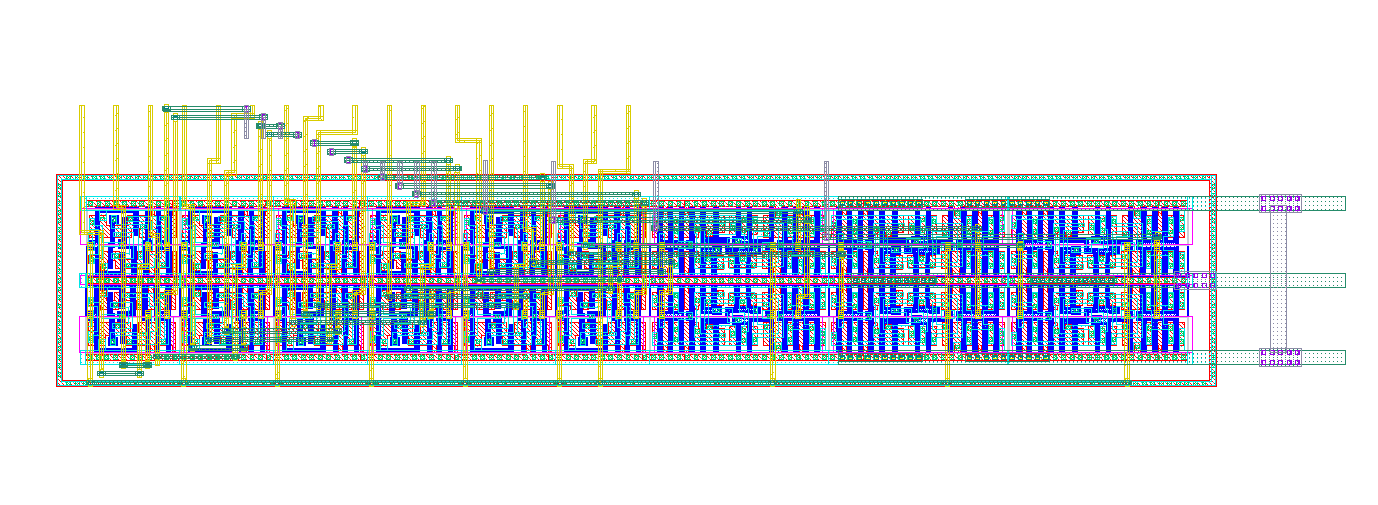
\includegraphics[width=\linewidth,height=2cm,keepaspectratio]{images/frida_capdriver.png}\\[2pt]
      {\tiny\fontsize{5}{5.5}\selectfont\lineskiplimit=-\maxdimen \textbf{Cap Drivers:}\\
      \textbullet~16-bit, scaled to caps\\
      \textbullet~$\sim$1\,ns settling\\}
    \end{column}
  \end{columns}
\end{frame}

%% ============================================================
%% Full ADC Layout (2D + 3D)
%% ============================================================
\begin{frame}
  \frametitle{Full ADC Layout}
  \begin{columns}
    \begin{column}{0.5\textwidth}
      \begin{center}
        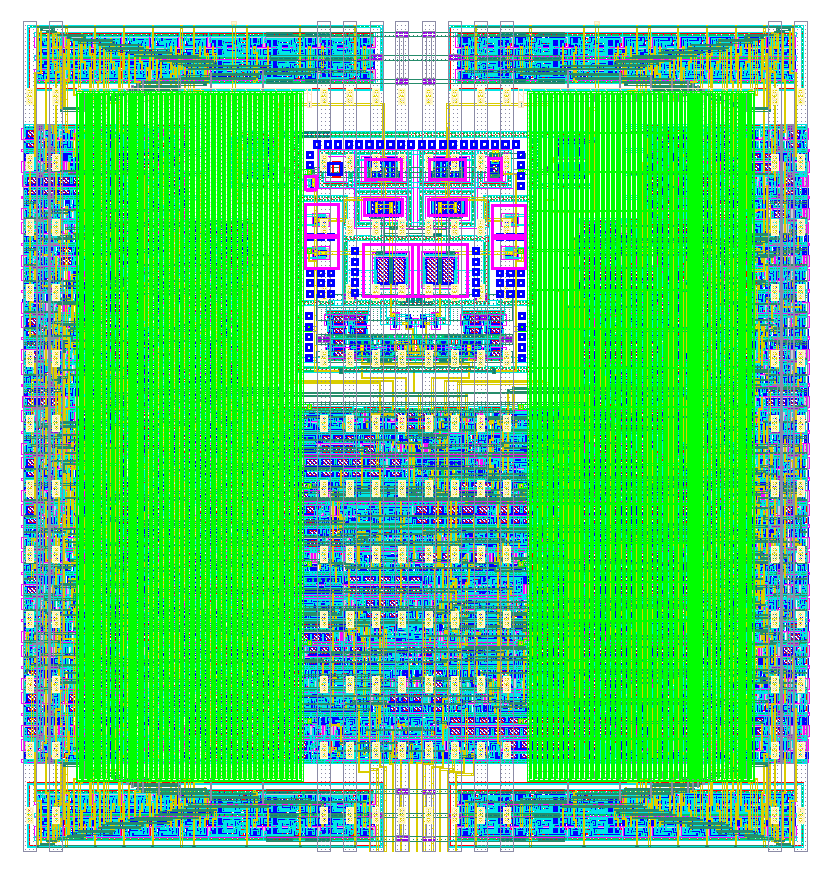
\includegraphics[width=0.95\linewidth,height=0.78\textheight,keepaspectratio]{images/frida_adc.png}\\[2pt]
        {\small 2D: 60$\times$60\,$\mu$m}
      \end{center}
    \end{column}
    \begin{column}{0.5\textwidth}
      \begin{center}
        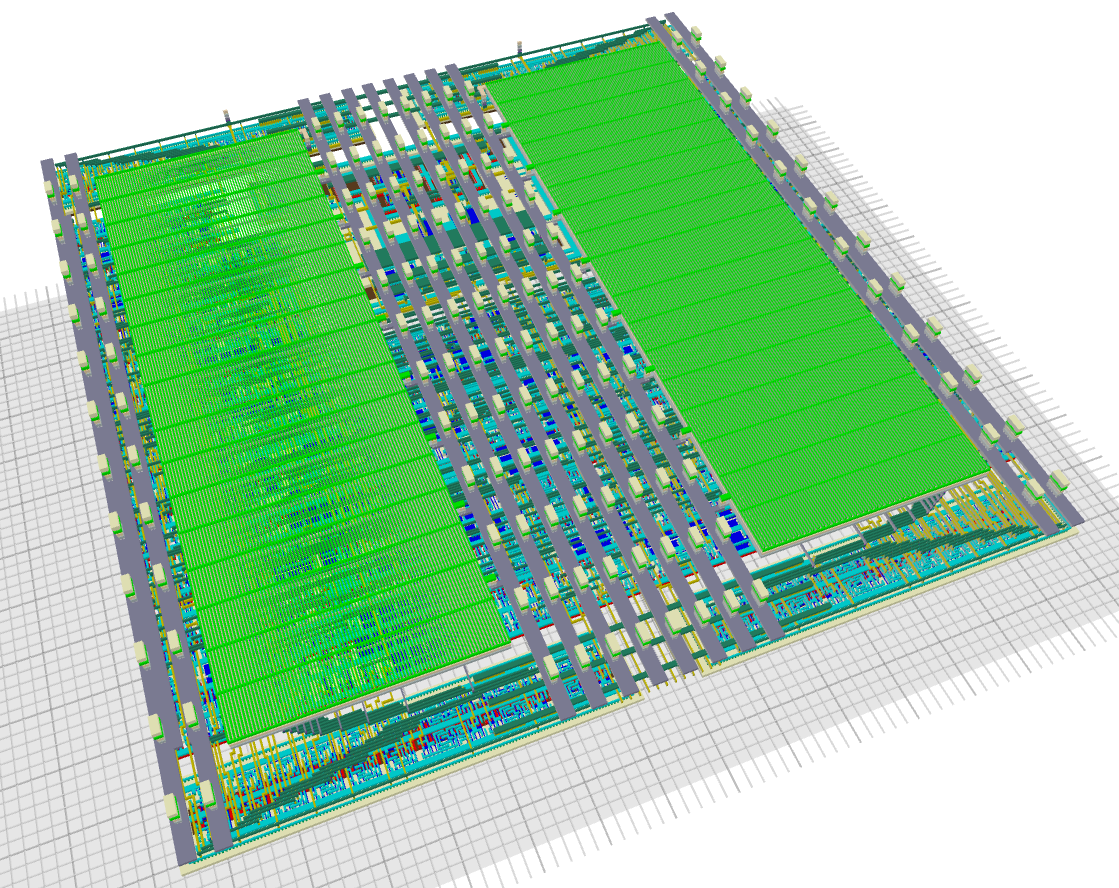
\includegraphics[width=0.95\linewidth,height=0.78\textheight,keepaspectratio]{images/frida_adc_3d.png}\\[2pt]
        {\small 3D view with CDAC arrays}
      \end{center}
    \end{column}
  \end{columns}
\end{frame}

%% ============================================================
%% Chip Comparison: IHP 130nm vs TSMC 65nm
%% ============================================================
\begin{frame}
  \frametitle{Prototype Chips}
  \begin{columns}[T]
    \begin{column}{0.48\textwidth}
      \begin{center}
        {\small \textbf{Initially designed w/ FOSS PDK \& tools:}}\\[4pt]
        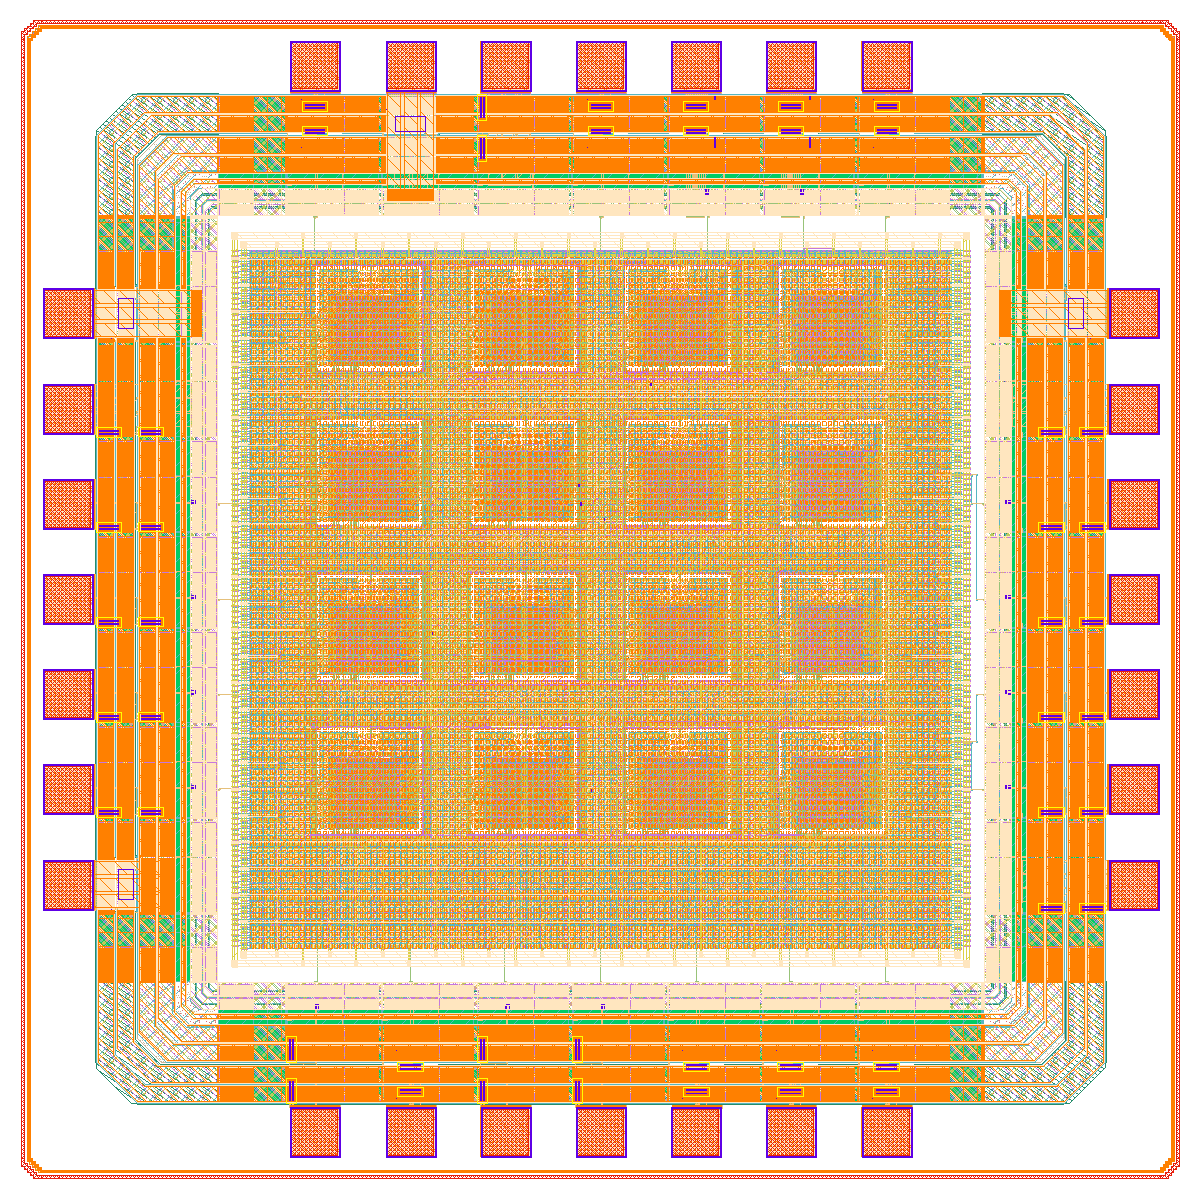
\includegraphics[width=\linewidth,height=0.65\textheight,keepaspectratio]{images/frida_130A.png}\\[2pt]
        {\small IHP SG13G2 (130\,nm) --- 1.6$\times$1.6\,mm}
      \end{center}
    \end{column}
    \begin{column}{0.48\textwidth}
      \begin{center}
        {\small \textbf{Ported for final submission:}}\\[4pt]
        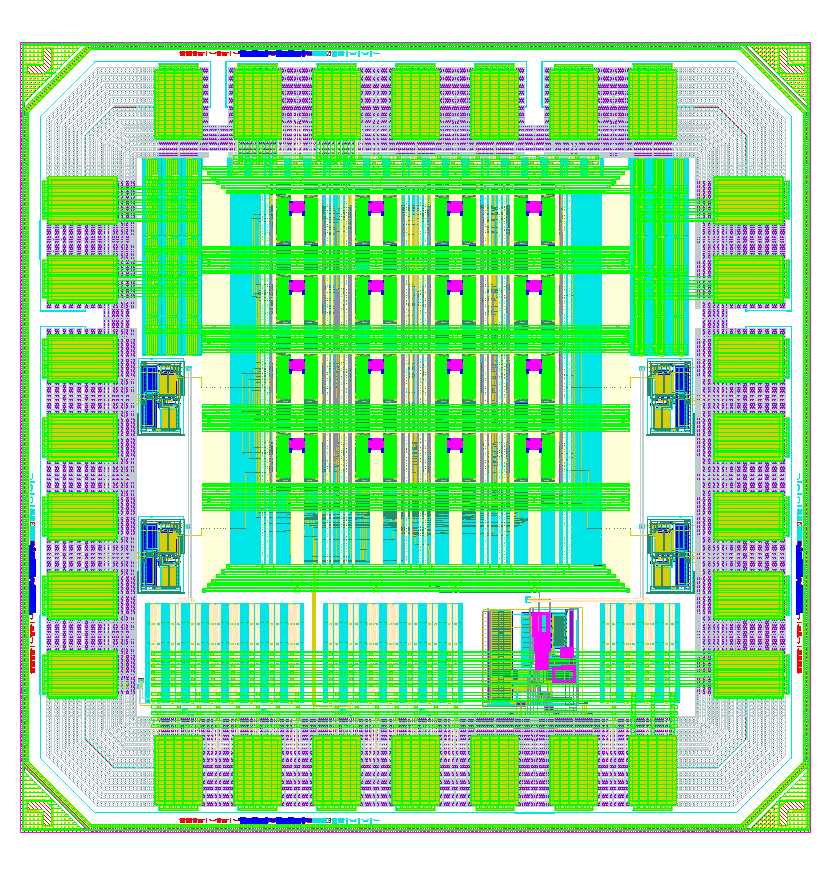
\includegraphics[width=\linewidth,height=0.65\textheight,keepaspectratio]{images/frida_65A.png}\\[2pt]
        {\small TSMC 65\,nm LP --- 1$\times$1\,mm}
      \end{center}
    \end{column}
  \end{columns}
  \begin{tikzpicture}[remember picture,overlay]
    \node[anchor=north east] at ([xshift=-0.3cm,yshift=-0.3cm]current page.north east)
      {
\includegraphics[width=1.2cm]{images/qr.png}};
  \end{tikzpicture}
\end{frame}

%% ============================================================
%% Outlook: Fabrication → Testing
%% ============================================================
\begin{frame}
  \frametitle{Outlook}
  \begin{tikzpicture}[remember picture,overlay]
    \node[anchor=center,xshift=-3.5cm,yshift=-1cm] at (current page.center)
      {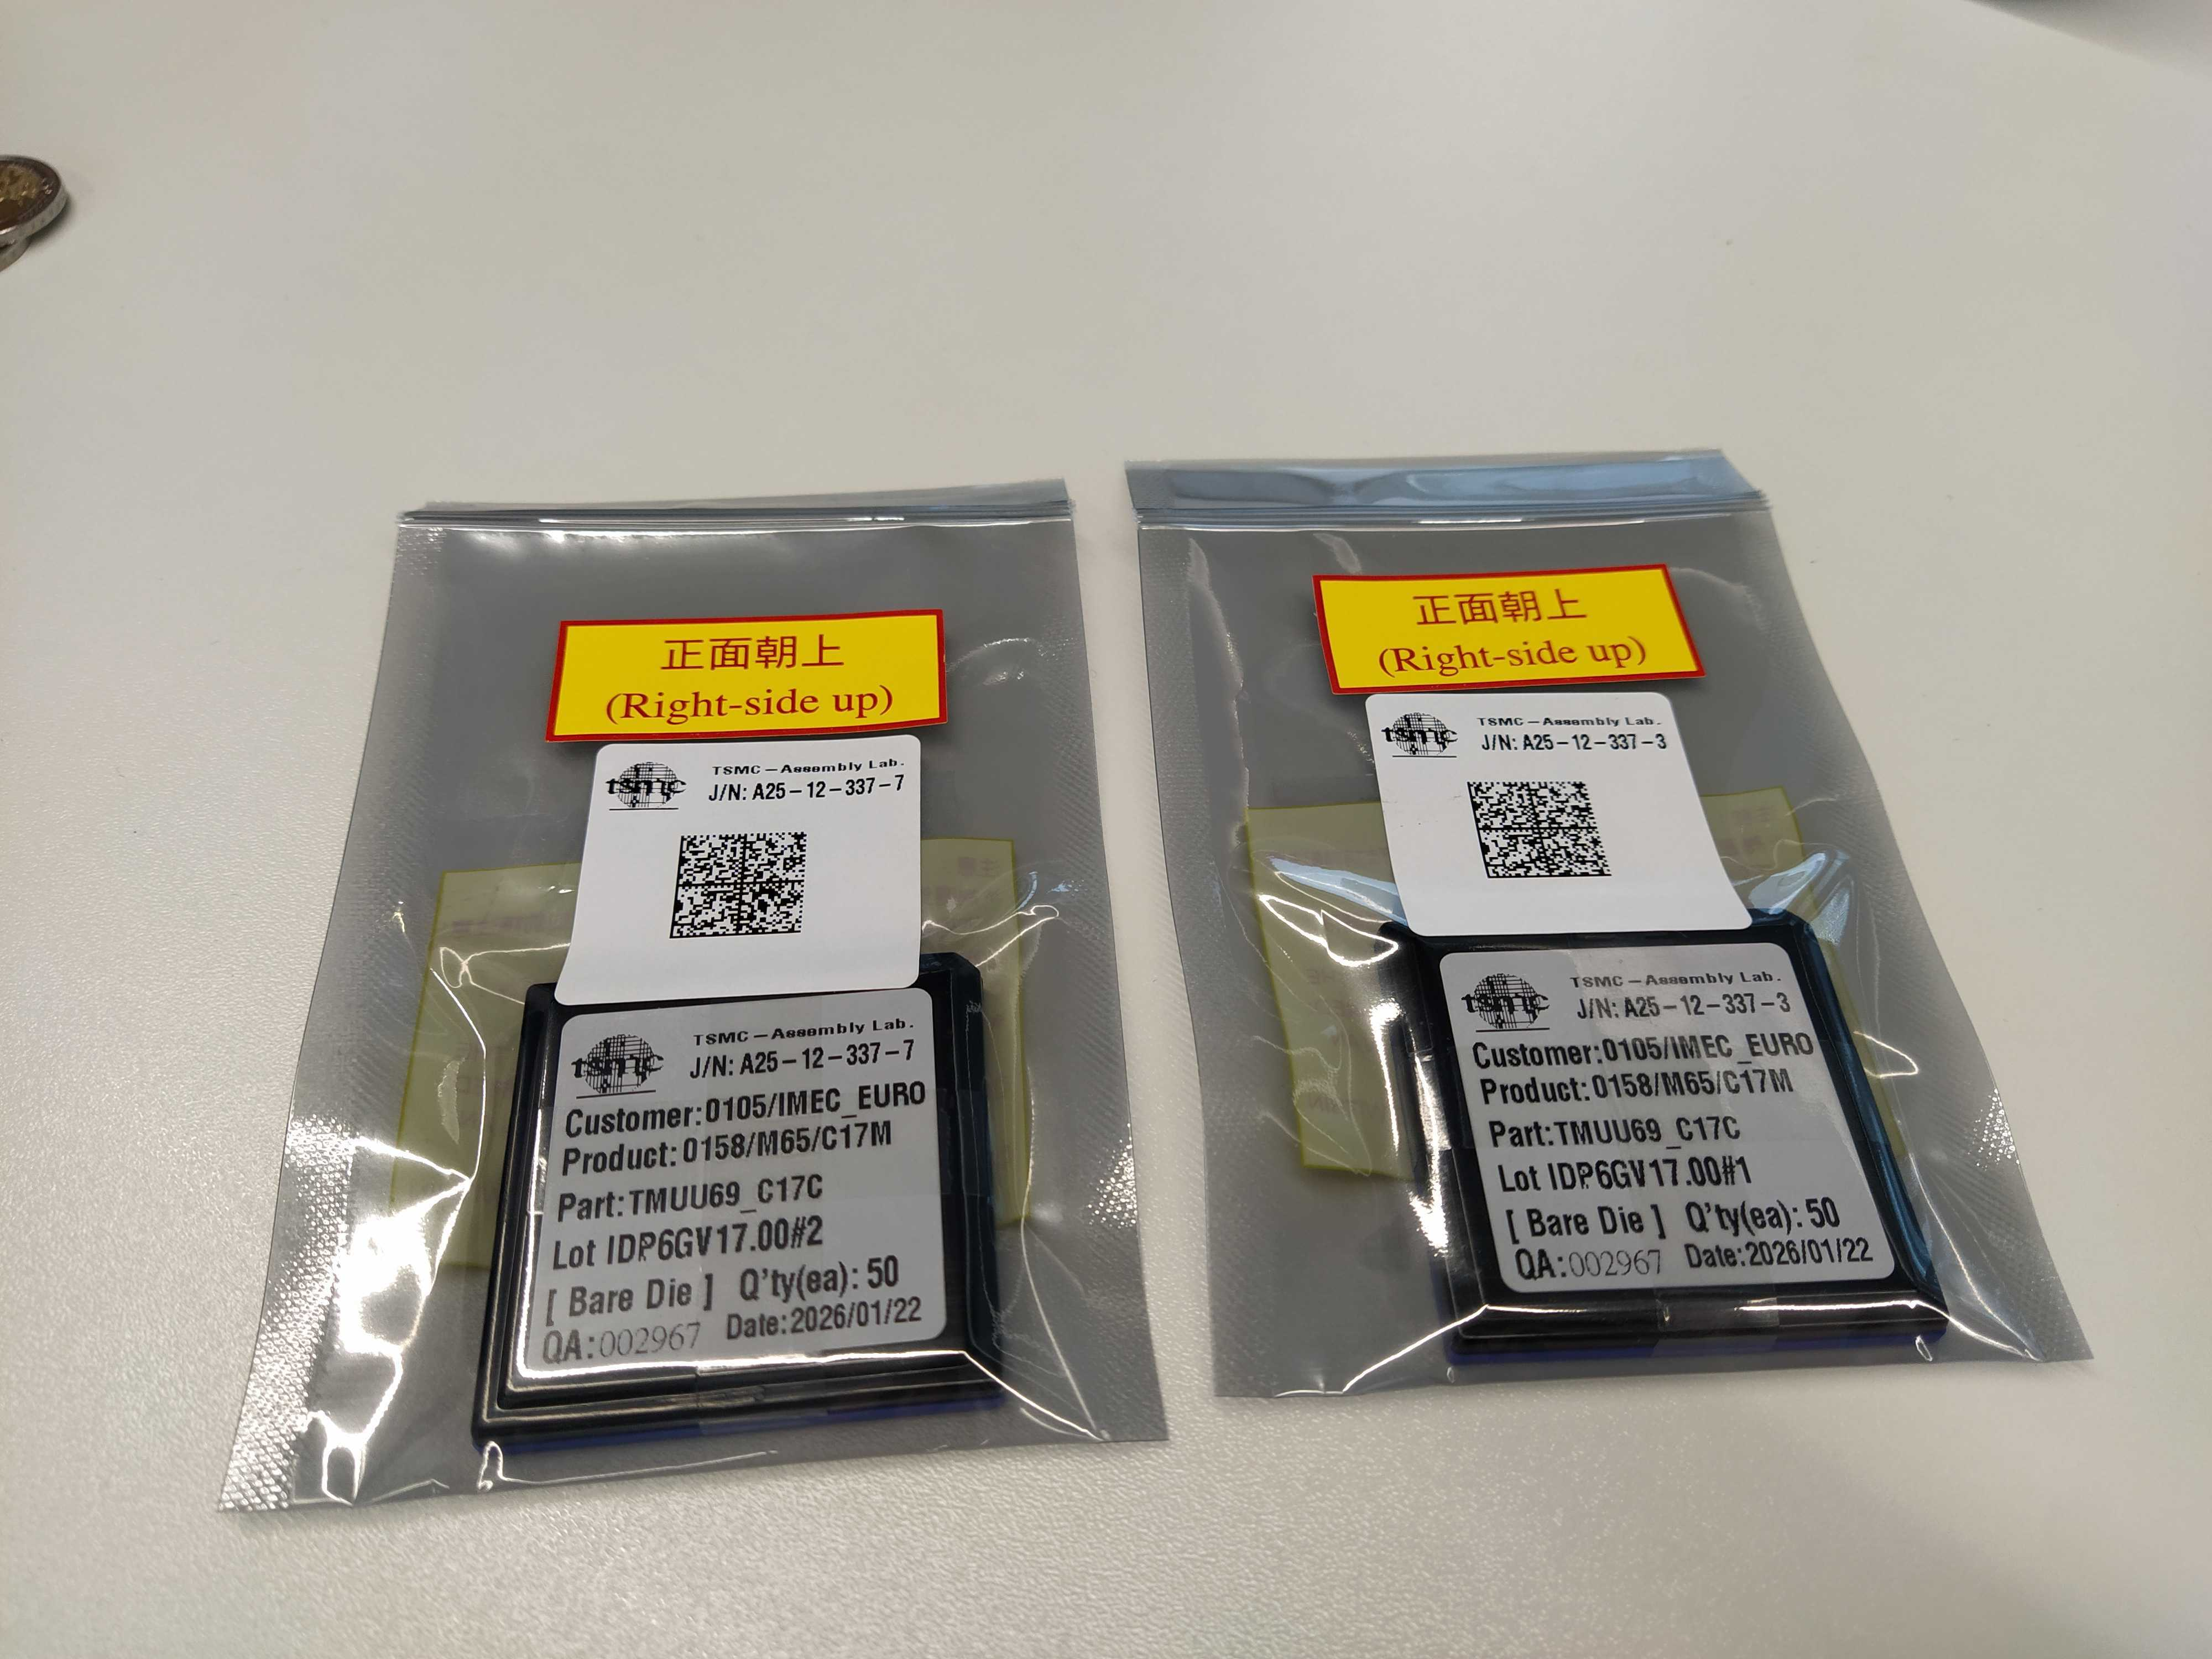
\includegraphics[height=0.50\textheight]{images/mail.jpg}};
    \node[anchor=center,xshift=3.8cm,yshift=-1cm] at (current page.center)
      {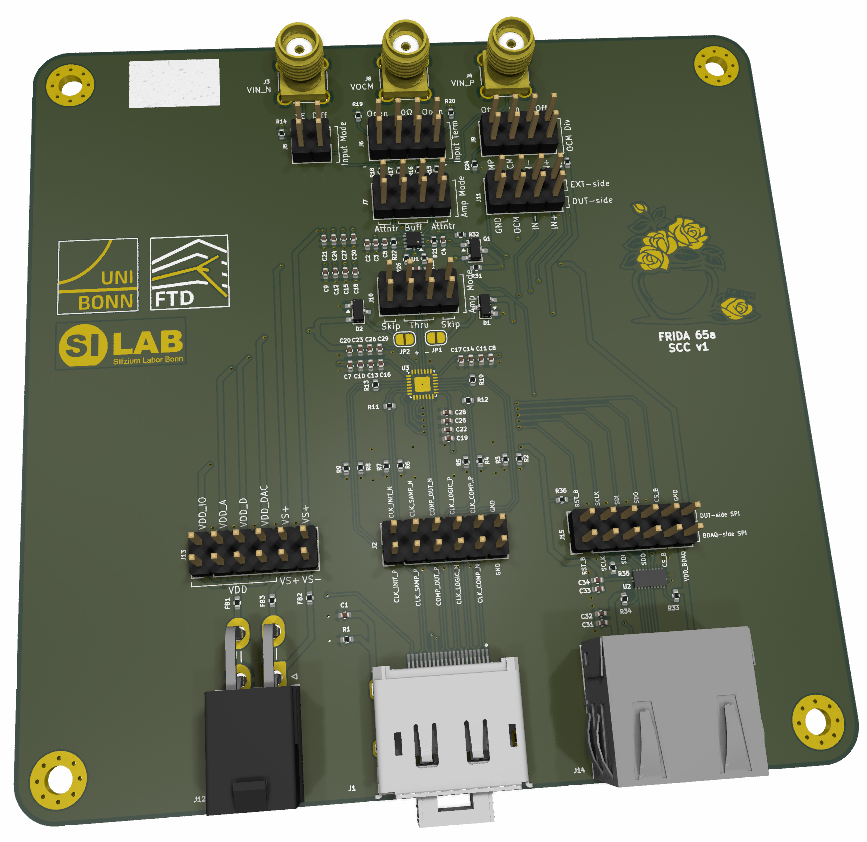
\includegraphics[height=0.60\textheight]{images/pcb_cropped.png}};
    \draw[-{Stealth[length=4mm]},line width=2pt,NordBlue]
      ([xshift=-0.3cm,yshift=-1cm]current page.center)
      -- ([xshift=0.8cm,yshift=-1cm]current page.center);
    \node[anchor=north east] at ([xshift=-0.3cm,yshift=-0.3cm]current page.north east)
      {
\includegraphics[width=1.2cm]{images/qr.png}};
    \node[anchor=north] at ([yshift=-1.5cm]current page.north)
      {\color{NordBody} \small 100 test ASICs received, ready for wirebonding on carrier board};
  \end{tikzpicture}
\end{frame}

\end{document}
